\chapter{How AI Systems ``Think'' (At the Level You Need)}

\epigraph{It is easier to be fooled by a confident answer than to recognize the difference between confidence and competence.}{Adapted from Daniel Kahneman}

\section{Prediction, Not Understanding}

The most important thing to understand about AI systems is that they do not understand anything in the way humans do.

When you ask an AI ``What is the capital of France?'', it is not retrieving a fact from memory like you would. It is predicting that, given that question pattern, ``Paris'' is the most likely next word based on billions of text examples it saw during training.

This distinction might seem academic, but it matters profoundly in practice:

\begin{itemize}
    \item The AI does not ``know'' whether its answer is correct
    \item It can produce plausible-sounding nonsense with the same confidence as accurate information
    \item It cannot verify its own outputs against reality
    \item Its level of confidence does not correlate with accuracy
\end{itemize}

Think of it this way: if you trained a parrot by exposing it to millions of business conversations, it might learn to say ``increase market penetration'' at contextually appropriate moments. The parrot sounds businesslike, but it has no concept of markets or penetration. The parrot predicts appropriate-sounding words based on patterns.

Large language models are vastly more sophisticated than parrots, but the fundamental principle holds. They predict statistically likely continuations. They do not understand meaning.

\begin{keyinsight}
AI generates predictions about what text should come next, not retrievals of knowledge or conclusions from reasoning. The output looks intelligent because it learned from intelligent text, not because the system thinks.
\end{keyinsight}

\section{Strengths You Can Rely On}

Understanding that AI operates through pattern prediction helps you identify what it does well. AI excels at tasks where statistical patterns in data lead to useful outputs.

\subsection{Pattern Matching at Scale}

AI can process enormous datasets to find patterns that would take humans weeks or months to identify:

\begin{itemize}
    \item \textbf{Finding similar items:} ``Show me all customer support tickets similar to this one''
    \item \textbf{Categorization:} Sorting thousands of documents into predefined categories
    \item \textbf{Anomaly detection:} Identifying expense reports that deviate from normal patterns
    \item \textbf{Trend identification:} Spotting recurring themes in customer feedback
\end{itemize}

\subsection{Text Transformation}

AI trained on text is excellent at reformatting, restructuring, and translating between styles:

\begin{itemize}
    \item \textbf{Summarization:} Condensing long documents into key points
    \item \textbf{Format conversion:} Turning meeting notes into action items, or bullet points into narrative paragraphs
    \item \textbf{Translation:} Converting between languages (with important caveats about accuracy)
    \item \textbf{Tone adjustment:} Making formal text casual, or technical text accessible
    \item \textbf{Data extraction:} Pulling structured information from unstructured text (names, dates, amounts)
\end{itemize}

\begin{realexample}[Document Summarization in Legal Review]
A legal team needed to review 500 contracts for specific clauses. Reading each contract would take weeks. Using AI to extract and summarize relevant sections reduced the first-pass review time by 75\%. Lawyers still verified every AI-identified clause, but the AI handled the time-consuming scanning work.
\end{realexample}

\subsection{Generation Within Familiar Patterns}

AI generates content that follows patterns it learned during training:

\begin{itemize}
    \item \textbf{Drafting standard documents:} Emails, reports, proposals, meeting agendas
    \item \textbf{Creating variations:} Multiple versions of marketing copy or product descriptions
    \item \textbf{Spreadsheet formulas:} Creating calculations, templates, and analysis structures
    \item \textbf{Brainstorming:} Generating ideas, options, or approaches to consider
\end{itemize}

The key phrase is ``within familiar patterns.'' AI generates text that resembles what it has seen before. It does not create genuinely novel solutions to unprecedented problems.

\subsection{Synthesis and Organization}

AI can combine information from multiple sources and impose structure:

\begin{itemize}
    \item \textbf{Creating outlines:} Organizing scattered information into logical structures
    \item \textbf{Combining perspectives:} Synthesizing multiple viewpoints into a coherent summary
    \item \textbf{Suggesting frameworks:} Proposing ways to categorize or organize data
\end{itemize}

\begin{table}[htbp]
\centering
\begin{tabularx}{\textwidth}{lXX}
\toprule
\textbf{Task Type} & \textbf{AI Strength Level} & \textbf{Verification Need} \\
\midrule
Format conversion & High & Low (structure is visible) \\
Summarization & High & Medium (check completeness) \\
Data extraction & High & Medium (spot-check accuracy) \\
Translation & Medium & High (nuance matters) \\
Factual answers & Medium & Very high (prone to errors) \\
Novel reasoning & Low & Critical (often fails) \\
\bottomrule
\end{tabularx}
\caption{AI capability levels and verification requirements}
\end{table}

\begin{figure}[htbp]
\centering
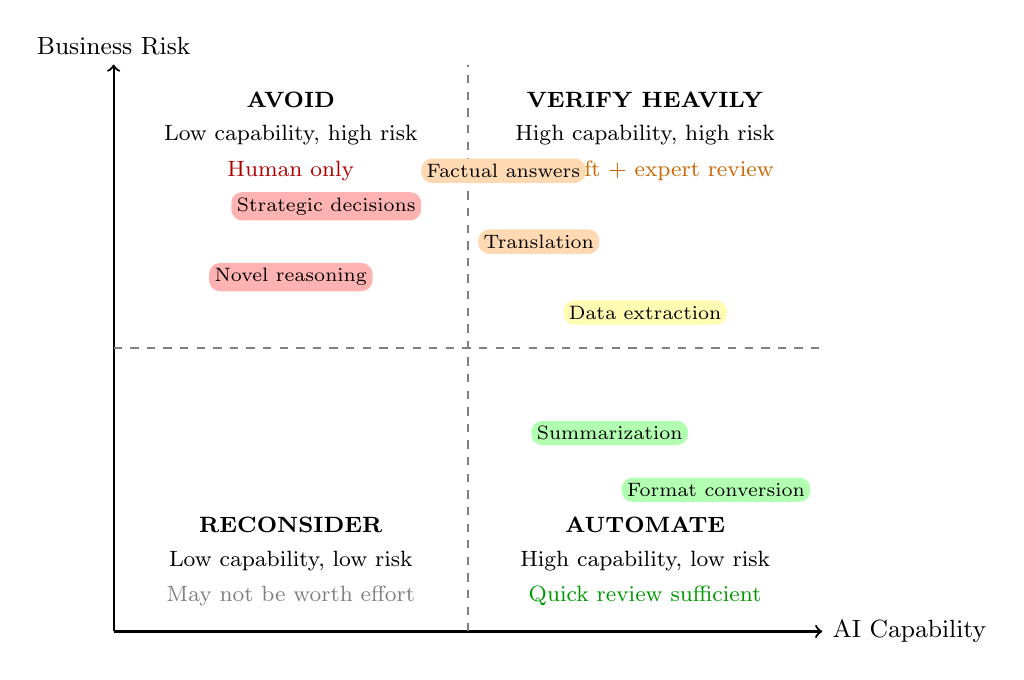
\begin{tikzpicture}[scale=0.9]
    % Draw axes
    \draw[thick, ->] (0,0) -- (10,0) node[right, font=\small] {AI Capability};
    \draw[thick, ->] (0,0) -- (0,8) node[above, font=\small] {Business Risk};

    % Quadrant labels
    \node[font=\footnotesize] at (2.5, 7.5) {\textbf{AVOID}};
    \node[font=\footnotesize] at (2.5, 7) {Low capability, high risk};
    \node[font=\footnotesize, text=red!70!black] at (2.5, 6.5) {Human only};

    \node[font=\footnotesize] at (7.5, 7.5) {\textbf{VERIFY HEAVILY}};
    \node[font=\footnotesize] at (7.5, 7) {High capability, high risk};
    \node[font=\footnotesize, text=orange!80!black] at (7.5, 6.5) {AI draft + expert review};

    \node[font=\footnotesize] at (2.5, 1.5) {\textbf{RECONSIDER}};
    \node[font=\footnotesize] at (2.5, 1) {Low capability, low risk};
    \node[font=\footnotesize, text=gray] at (2.5, 0.5) {May not be worth effort};

    \node[font=\footnotesize] at (7.5, 1.5) {\textbf{AUTOMATE}};
    \node[font=\footnotesize] at (7.5, 1) {High capability, low risk};
    \node[font=\footnotesize, text=green!60!black] at (7.5, 0.5) {Quick review sufficient};

    % Quadrant dividers
    \draw[dashed, gray] (5,0) -- (5,8);
    \draw[dashed, gray] (0,4) -- (10,4);

    % Plot tasks
    \node[fill=green!30, rounded corners, font=\scriptsize, inner sep=2pt] at (8.5, 2) {Format conversion};
    \node[fill=green!30, rounded corners, font=\scriptsize, inner sep=2pt] at (7, 2.8) {Summarization};
    \node[fill=yellow!30, rounded corners, font=\scriptsize, inner sep=2pt] at (7.5, 4.5) {Data extraction};
    \node[fill=orange!30, rounded corners, font=\scriptsize, inner sep=2pt] at (6, 5.5) {Translation};
    \node[fill=orange!30, rounded corners, font=\scriptsize, inner sep=2pt] at (5.5, 6.5) {Factual answers};
    \node[fill=red!30, rounded corners, font=\scriptsize, inner sep=2pt] at (2.5, 5) {Novel reasoning};
    \node[fill=red!30, rounded corners, font=\scriptsize, inner sep=2pt] at (3, 6) {Strategic decisions};

\end{tikzpicture}
\caption{AI Task Selection Matrix: Match task type to appropriate oversight level}
\label{fig:ai-task-matrix}
\end{figure}

\section{Common Limitations and Failure Modes}

AI fails in predictable ways. Knowing these failure modes helps you avoid costly mistakes.

\subsection{Hallucinations}

AI will confidently state false information. It might cite papers that do not exist, attribute quotes to people who never said them, or describe features that products do not have. This happens because the AI is generating plausible-sounding text, not retrieving verified facts.

\begin{warning}[The Fake Case Citation Disaster]
In 2023, lawyers submitted a legal brief to federal court that cited multiple precedent cases. The cases sounded legitimate. The citations looked correct. The problem: none of the cases existed. They were AI hallucinations. The AI generated plausible-looking legal citations because it had learned the pattern of how citations look, but it did not have access to actual case law. The lawyers faced sanctions for not verifying the AI output.
\end{warning}

This was not a rare edge case. Hallucinations are a fundamental characteristic of how these systems work. They generate probable text, not verified facts.

\subsection{Outdated Information}

AI training has a cutoff date. Models do not know about events, products, regulations, or changes after that date. If you ask about something recent, you will get information about the state of the world at training time, stated as if it were current.

\begin{realexample}[The Product Feature Confusion]
A product manager asked an AI assistant about features in a competitor's software. The AI confidently described the pricing tiers and capabilities. The manager created a competitive analysis based on this information. At the next executive meeting, it became clear the analysis was wrong---the competitor had completely restructured their offering six months earlier. The AI had described the old product structure because its training data predated the change.
\end{realexample}

For any question about current events, recent products, or time-sensitive information, verify against authoritative sources.

\subsection{Reasoning Failures}

AI struggles with tasks requiring genuine logic, especially:

\begin{itemize}
    \item \textbf{Multi-step reasoning:} Problems that require holding intermediate results and building on them
    \item \textbf{Arithmetic:} Surprisingly, AI often fails at basic math despite fluency with numbers
    \item \textbf{Constraint satisfaction:} Problems with hard requirements (e.g., scheduling with mandatory conditions)
    \item \textbf{Novel puzzles:} Anything that requires reasoning patterns not seen in training
\end{itemize}

Ask an AI to count the words in a sentence, and it frequently gets it wrong. Ask it to solve a logic puzzle, and it may produce an answer that violates the stated constraints.

\subsection{Bias Amplification}

AI learns from data. If the data reflects biases---and it almost always does---the AI will reproduce and sometimes amplify those biases.

\begin{warning}[Resume Screening Bias]
A major technology company developed an AI tool to screen resumes. The system learned from historical hiring data, which showed that the company had hired more men than women in technical roles. The AI learned to downgrade resumes from candidates who attended women's colleges or participated in women's technical organizations. The bias in historical data became bias in the AI's recommendations. The company abandoned the tool after discovering this.
\end{warning}

This is not fixable by ``removing bias from the AI.'' The bias is in the patterns the AI learned. Addressing this requires carefully evaluating whether patterns in training data reflect real quality differences or historical discrimination.

\subsection{Document Length Limitations}

AI can only consider a limited amount of text at once---typically equivalent to 20-100 pages, depending on the system. Think of it like working with a colleague who can only keep a certain number of pages in front of them at any time. For longer documents:

\begin{itemize}
    \item Information at the beginning or end may receive less attention
    \item The AI might miss connections between points discussed far apart in the document
    \item Summaries may emphasize some sections while neglecting others
\end{itemize}

If you need analysis of a 300-page annual report, understand that the AI cannot review all of it simultaneously. You may need to break the analysis into sections or focus on specific chapters.

\section{Why Answers Change}

The same prompt can produce different answers. This surprises people expecting software-like determinism. Understanding why this happens helps you decide when variability is acceptable and when it is problematic.

\subsection{Creativity Settings}

Most AI systems have a setting that controls how creative versus consistent the output is---vendors call this ``temperature'' but think of it as a creativity dial. Higher settings mean more variability and creative outputs. Lower settings mean more consistent, predictable results.

For strategic brainstorming or generating multiple marketing angles, you want more creativity. For extracting data from contracts or producing standardized reports, you want consistency. Some enterprise tools let you adjust this; others handle it automatically based on your task.

\subsection{System Updates}

AI providers regularly update their models. Your prompt that worked perfectly last month might produce different results after an update. This is both good (capabilities improve) and bad (workflows break).

\subsection{Context Differences}

The conversation history affects responses. The same question asked in isolation versus asked after a long discussion about a specific topic will get different answers because the AI treats the prior conversation as context.

\subsection{Prompt Phrasing}

Minor wording changes can significantly shift outputs. ``Summarize this'' versus ``What are the key points?'' might produce substantially different results, even though the intent seems similar.

\begin{table}[htbp]
\centering
\begin{tabularx}{\textwidth}{lXX}
\toprule
\textbf{Business Scenario} & \textbf{Variability} & \textbf{How to Manage} \\
\midrule
Marketing brainstorming & High (desirable) & Use creative settings \\
Contract data extraction & Low (required) & Use consistent settings, standardized prompts \\
Competitive analysis & Medium & Test multiple times, compare outputs \\
Executive summaries & Medium & Specify desired structure/format \\
Report generation & Medium & Provide detailed templates \\
\bottomrule
\end{tabularx}
\caption{Managing output variability by business use case}
\end{table}

\begin{tip}[Standardizing Critical Workflows]
For business processes where consistency matters---contract review, data entry, customer communications---develop standardized prompts and test them extensively. Small variations in phrasing can create large differences in output. Once you find a prompt that works reliably, document it and use it consistently.
\end{tip}

\section{The Verification Imperative}

Because AI can be confidently wrong, verification is not optional. Every AI output needs human review before you:

\begin{itemize}
    \item Send it to customers
    \item Include it in reports
    \item Base decisions on it
    \item Publish it externally
    \item Use it for legal or financial purposes
\end{itemize}

The depth of verification should match the stakes. Low-stakes tasks (internal brainstorming notes) require quick sanity checks. High-stakes tasks (legal documents, financial analysis, customer-facing content) require thorough review.

\begin{framework}[Verification Depth Decision Matrix]
Choose your verification approach based on two factors:

\textbf{Stakes:} What happens if the output is wrong?
\begin{itemize}
    \item Low: Minor inconvenience, easily corrected
    \item Medium: Significant time wasted, some reputational risk
    \item High: Financial loss, legal exposure, major reputation damage
\end{itemize}

\textbf{Reversibility:} How hard is it to fix mistakes after the fact?
\begin{itemize}
    \item Easy: Can edit or retract quickly
    \item Moderate: Requires communication and rework
    \item Hard: Once published, cannot effectively retract
\end{itemize}

\begin{tabular}{lll}
\toprule
\textbf{Stakes} & \textbf{Reversibility} & \textbf{Verification Level} \\
\midrule
Low & Easy & Quick scan for obvious errors \\
Low & Hard & Careful reading \\
Medium & Easy & Detailed review of key claims \\
Medium & Hard & Thorough fact-checking \\
High & Any & Complete verification, expert review \\
\bottomrule
\end{tabular}
\end{framework}

\begin{realexample}[Email Draft Verification]
A business development team uses AI to draft initial responses to partnership inquiries. Their verification process:

\begin{enumerate}
    \item AI drafts the email based on inquiry details and company guidelines
    \item Team member reads the draft and checks:
    \begin{itemize}
        \item Tone is appropriate
        \item No confidential information included
        \item Claims about capabilities are accurate
        \item Contact information is correct
    \end{itemize}
    \item Team member edits as needed and sends
\end{enumerate}

This takes 2-3 minutes versus 15 minutes to write from scratch. The verification is quick because email mistakes are easy to correct with follow-up messages. The same team would never use unverified AI output for contract terms, where stakes and irreversibility are both high.
\end{realexample}

\section{What You Do Not Need to Learn}

Many people believe they need to understand AI deeply to use it effectively. This is false. You do not need to understand combustion chemistry to drive a car.

\subsection{What You Do NOT Need}

\begin{itemize}
    \item How the underlying technology works mathematically
    \item Technical architecture details
    \item How AI systems are trained or optimized
    \item Configuration and tuning parameters
    \item The technical differences between vendors (GPT-4, Claude, Gemini, etc.)
    \item Engineering concepts like backpropagation or tensors
    \item Model customization techniques (unless pursuing enterprise-scale custom AI)
\end{itemize}

These topics are fascinating if you are interested in AI research or technology strategy. For day-to-day business use, they are not necessary.

\subsection{What You DO Need}

\begin{itemize}
    \item \textbf{Capability awareness:} What AI is good and bad at
    \item \textbf{Effective prompting:} How to structure requests for better results
    \item \textbf{Verification skills:} When to trust output and when to dig deeper
    \item \textbf{Output evaluation:} Recognizing hallucinations, bias, and logical errors
    \item \textbf{Risk assessment:} Understanding privacy, security, and accuracy implications
\end{itemize}

Think of it as the difference between an automotive engineer (who designs engines) versus a fleet manager (who needs to know how to evaluate vehicles, manage maintenance schedules, and optimize operations). You are the fleet manager, not the engineer.

\begin{keyinsight}
The right mental model for business leaders: AI is a powerful tool with known strengths and limitations. You need to understand those characteristics well enough to deploy the tool effectively and safely. You do not need to understand how the tool is built.
\end{keyinsight}

\section{Summary}

AI systems do not think or understand. They predict statistically likely outputs based on patterns in training data. This makes them excellent at pattern matching, text transformation, and generation within familiar domains. It also makes them prone to hallucinations, outdated information, reasoning failures, and bias amplification.

The same prompt can produce different outputs due to temperature settings, system updates, context differences, and prompt phrasing. Variability is sometimes desirable (creativity) and sometimes problematic (consistency-critical tasks).

Every AI output requires verification. The depth of verification should match the stakes and reversibility of the task. Quick scans suffice for low-stakes internal work. Thorough fact-checking is mandatory for high-stakes external communications.

You do not need to understand the technical internals of AI to use it effectively. You need to understand what it does well, where it fails, and how to verify its outputs.

With this mental model in place, you can make better decisions about when to use AI, how to structure your requests, and when to trust the results. The next chapter examines the fuel behind every AI system: data.

\begin{exercise}
Test an AI system with the following prompts and observe the failure modes:

\begin{enumerate}
    \item Ask for citations to academic papers on a specific niche topic. Check if the papers exist.
    \item Ask about a recent event (within the last few months). See if it acknowledges its knowledge cutoff.
    \item Ask it to solve a simple logic puzzle. Check if the answer violates any stated constraints.
    \item Ask the same question three times with slight rephrasing. Note the variability in responses.
\end{enumerate}

Document what you observe. This hands-on experience with failure modes is more valuable than reading about them.
\end{exercise}

\begin{exercise}
For your own role, create a verification checklist for AI-generated content. List the specific things you would check before using AI output for:

\begin{itemize}
    \item Internal team communications
    \item Client-facing documents
    \item Financial or legal content
    \item Social media posts
\end{itemize}

Keep this checklist handy. You will use it.
\end{exercise}
